\documentclass[../main.tex]{subfiles}

\begin{document}


\section{Theoretical performance}
\label{section:analysis:theoric_performance}
\begin{figure}[h]
    \centering
    \makebox[\textwidth][c]{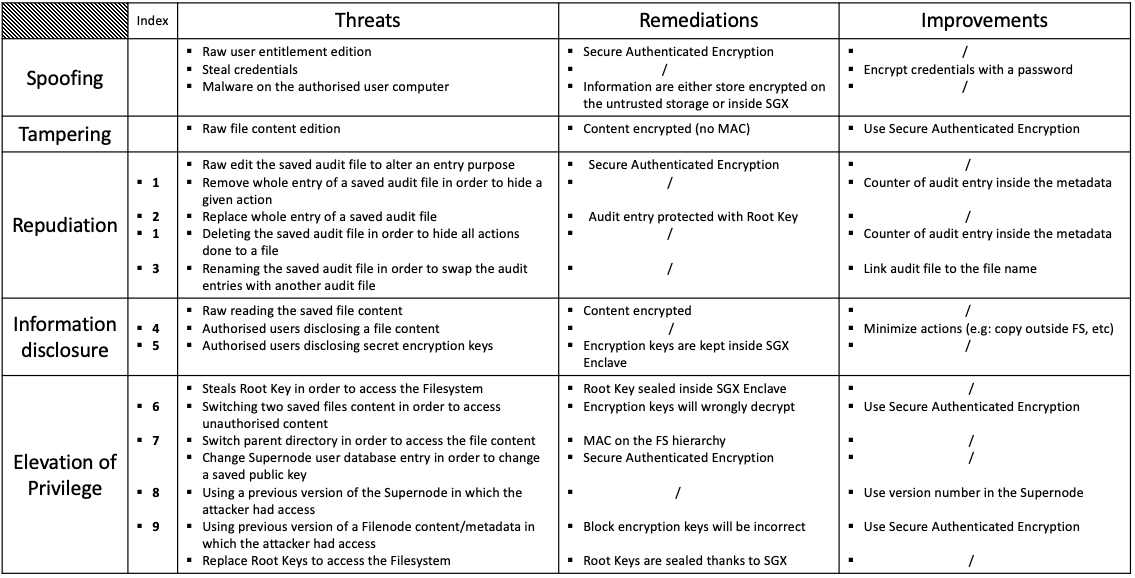
\includegraphics[width=1.25\textwidth]{images/analysis/security_assessment}}
    
    \caption{Security assessment}
    \label{figure:analysis:security_assessment}
\end{figure}
\par The above Figure \ref{figure:analysis:security_assessment} shows the security assessment of LAUXUS based on the theoretical description seen in the Chapter \ref{chapter:lauxus}. We based our table on the STRIDE model as explained in the problem statement. As we can see from the table, we aren't protected against all the listed threats. This is why we added an improvement column to explain what can be done to mitigate the concerned threat in a future LAUXUS version. As some of the threats and remediation are straightforward to understand, we will only focus on the harder ones that are indexed to ease the following explanations:
\begin{itemize}
    \item[\textbf{(1)}] As audit entries are self standing (cfr. Section \ref{section:lauxus:audit}), there is no linkage between the entries inside the audit file. Which means that if an attacker can precisely remove a whole entry, nobody will be able to note the modification. Note that this is not an easy task for the lambda attacker as the entries are not fixed size (depends on the length of the purpose), however if the attacker knows the length of the original purpose, it becomes trivial. Multiple remediation\footnote{Store the audit keys inside the metadata structure, Hash of the whole plaintext file} are possible but the most efficient one is to include the number of audit entry inside the metadata structure. This allows to keep an excellent audit entry write overhead while solving the issue. Indeed, the whole metadata structure is written anyway to disk.
    \item[\textbf{(2)}] In the same manner as the attack \textbf{(1)}, an attacker could replace a while entry with another one (e.g: generated from another LAUXUS instance). Even if it seems feasible, we must not forget that each audit entry is protected thanks to the audit root key. As root keys are unique to each LAUXUS instance, it becomes impossible for an attacker to forge a valid audit entry.
    \item[\textbf{(3)}] An attacker could rename an audit entry to another one in order to swap the audit entries. Currently, our implementation is vulnerable to this attack. Indeed, inside the audit file, there is no link to the concerned file. To solve this, we just need to bind the two files together. An easy way to do so is to add a small section at the beginning of each audit file. This section contains the name or the UUID of the concerned file. This section must be encrypted using the key stored in the cryptographic context of the corresponding metadata structure. We can't use the root key as the encryption key as an attacker would only need to swap the section with another audit file. This process is very efficient as the new section must only be written once (at the corresponding file creation).
    \item[\textbf{(4)}] As discussed in the threat model, once an authorised user can access a certain version of the Filesystem, we can't do anything to protect this version if the user choose to make this information public. However, if we can control the OS, we can prevent the user from copying the decrypted content outside the system. This will prevent the user from sharing it. However, it can only be done to a certain extent, the user can still take a picture of the decrypted content.
    \item[\textbf{(5)}] Similarly to the point \textbf{(4)}, an malicious authorised user may wish to share the encryption keys with other unauthorised user. In a classical scenario, this would be impossible to prevent. Fortunately, thanks to SGX secure computation, we hide all the encryption keys to the user, preventing them from disclosing them.
    \item[\textbf{(6)}] In order to access the content of a file an authorised user has not access to, the user may want to switch the saved file content with another file to which he has access. In a nutshell, given two files A and B in which user X can access file A, user X may want to access file B. The idea is to switch the content of file A and B but keeping the correct metadata structure (and thus the user entitlement). With our implementation, nothing will be noticed if the two files have the same number of blocks. Indeed, the block keys are stored inside the metadata structure, so LAUXUS will just read a file block and decrypt it using the corresponding block key. However, as the key is incorrect, the content will be wrongly decrypted but without throwing any error. To improve this, we can use an authenticated encryption algorithm to throw the error. Using an authenticated algorithm will also enable the possibility to use forensic (warns the administrator of inappropriate behaviour). Furthermore, with this forensic, we know on which computer the inappropriate action has been done.
    \item[\textbf{(7)}] Similarly to the attack \textbf{(6)}, an attacker may change the parent directory of file to one that he is allowed to access. This process is impossible thanks to the authenticated encryption on the metadata structure. Indeed, even if the parent directory is in plaintext (in fact, it is the children nodes that are in plaintext), the information is protected as it is passed as the Authenticated Additionnal Data inside the GCM encryption algorithm.
    \item[\textbf{(8)}] An attacker could use a previous version of the supernode. A version in which he was allowed to access the filesystem. Our implementation doesn't cope with this threat however a solution is possible. We can use a simple version number on the Supernode. Each time the Supernode is updated, this version number increases. However this is not enough, we must also link the Filenodes and Dirnodes to this version number. Consequently, each node will also have a version number. However, the node version number will only be updated with the one of the Supernode whenever the node is accessed. Furthermore, a user can only access a node if the node's version is smaller or equals to the Supernode version. This process may seem imperfect because nodes version are only updated when they are accessed. Let's demonstrate this with a simple scenario:
    \par We consider Alice and Bob, both can access version 1 of the Supernode. Alice decides to revoke Bob creating a new Supernode with version 2. At this time, Bob can still access the filesystem and all the files he used to access by simply using the previous version of the Supernode. This is not a security issue because Bob had already access to these files. When Alice choose to edit a file X, it will assign a new version to this file. Now, Bob can no longer do the same trick and don't know the new version of the file because its Supernode version is lower than the version of file. This scenario proves the effectiveness of our process.
    \item[\textbf{(9)}] Similarly to the attack \textbf{(8)}, an attacker may use previous version of the metadata or the content of a file. This idea behind this action is to use the old user entitlement (where he has access to the file) and combine it with the new version of the content (which he should not have access to because he has been revoked). The protection is similar to the one seen in the attack \textbf{(6)}.
\end{itemize}

\par After analyse our model, we can clearly conclude that: once a user has access to a version x of a file, he will always be able to access this version of the file (through the different attack seen above). Furthermore, in the case the end-user computer is hacked, the attacker can only access the content that the targeted user can access, which may be very small (and at the condition that the user credentials are in plaintext). This means that our model is relatively strong against a Man-In-The-Computer attacker.
\par As we have seen from the above description, although our theoretical model is quite complicated, it still has some flows. However, these flows are not so complicated to fix and can be implemented in a small amount of time. The flexibility of our code base makes this tasks even more easy.

\end{document}